\documentclass{article}

\usepackage{graphicx} % Image management
\usepackage{listings} % Source code management
\usepackage[sorting=none]{biblatex} % Biblio managment

\addbibresource{biblio.bib}

\begin{document}

\title{PSAT - Prépublication}
\author{BAILLY Grégoire \\ CHATELIN Corentin \\ GIRAUD Corentin \\ TOULIER-ANCIAN Lucas \\ VIRY Baptiste }

\maketitle

\begin{abstract}
%apprentissage automatique
%Réseau de neurone \\
%Apprentissage fédéré \\
%qlq application \\
%Rappel de la problématique

Les personnes victimes d'un AVC sont considérées comme étant à risque dans la suite de leur vie quotidienne, et peuvent être sujettes à de nombreux problèmes graves arrivant parfois sans signes avant-coureurs. Il est donc important de permettre à ces personnes d'accéder à un suivi strict et constant de leur quotidien, afin d'obtenir une réaction rapide des services de santé en cas de détection de problèmes. Comment donc permettre un suivi "strict et constant" tout en se conformant aux contraintes qu'impliquent des données de santé ? Nos téléphones intelligents, tous équipés de capteurs gyroscopiques, ainsi que d'accéléromètres, offrent une solution intéressante. L'objet de cette étude est de parvenir à mettre en place un prototype d'application basée sur l'apprentissage fédéré sur mobile avec l'aide de modèles de reconnaissances d'activité humaine. Ainsi, chaque téléphone intelligent entraînera/raffinera un modèle sur les données de l'utilisateur, évitant ainsi l'envoi de données sensibles à un serveur centralisé. Le serveur agrégera ensuite les contributions de chacun des utilisateurs sans connaître l'influence de ces derniers dans la mise à jour du modèle.

\end{abstract}

\section{État de l'art}

\subsection{Introduction}
Le but de notre cas d'étude est de réaliser une prédiction d'une suite d'activités exercées par un patient sur un laps de temps donné. Les activités que nous tentons de prédire sont: la marche à pied sur sol plat, la montée d'escalier, la descente d'escalier, la position immobile assise, la position immobile debout et la position allongée.
Afin de réaliser ces prédictions, nous utiliserons un réseau de neurones entraîné sur deux jeux de données:
\begin{itemize}
    \item \underline{HAR Dataset}: qui inclut des données accélérométriques et gyroscopiques en fonction du temps à partir d'un Samsung Galaxy SII pour 30 personnes (de 19 à 48 ans). \cite{AnguitaPublicDomainDataset2013}
    \item \underline{MotionSense}: qui inclut des données accélérométriques et gyroscopiques en fonction du temps à partir d'un iPhone 6S pour 24 personnes. \cite{MalekzadehMobileSensorData2019} \cite{MalekzadehPrivacyUtilityPreserving2019}
\end{itemize}
Un serveur Linux hébergera une API en charge de la distribution du réseau de neurones et de la mise à jour de ce dernier à partir de l'entraînement du modèle sur les téléphones clients.

\subsection{L'apprentissage fédéré}

L'apprentissage fédéré (\textit{federated learning} en anglais) consiste à entraîner un algorithme sur la machine des utilisateurs d'une application et à partager les apprentissages réalisés sur la machine de chaque utilisateur. Dans notre cas, nous tenterons d'entraîner un réseau de neurones de manière décentralisée et sécurisée.

\subsubsection{Processus traditionnel dans une architecture client/serveur}

Dans une architecture client / serveur, la manière traditionnelle d'utiliser un modèle pour faire des prédictions est résumé dans le schéma ci-dessous et suit le processus suivant:

\begin{enumerate}
    \item Le client fait une requête au serveur pour demander des prédictions sur des données qu'il joint à la requête.
    \item Le serveur utilise son modèle local pour faire des prédictions sur les données du client qu'il stocke.
    \item Le serveur renvoie les prédictions au client qui les affiche à l'utilisateur.
    \item Ce dernier peut alors juger de la pertinence des résultats et corriger les prédictions si nécessaire. Il renvoie alors la correction des prédictions au serveur.
    \item Le serveur stocke de nouveau la correction des prédictions qu'il utilisera par la suite pour entraîner de nouveau le modèle.
\end{enumerate}

\centerline{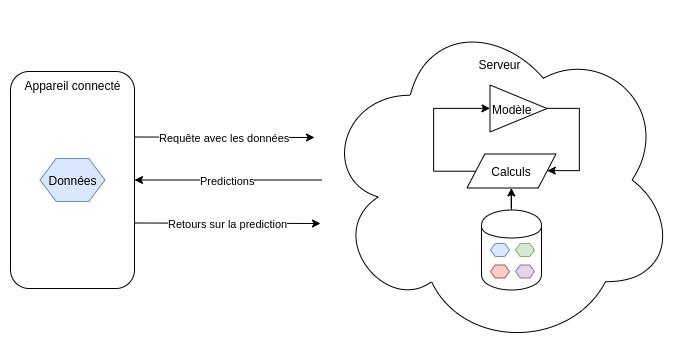
\includegraphics[width=14cm]{centralize.png}}

Néanmoins, les inconvénients de ce processus sont nombreux. En effet, dans le contexte des applications mobiles, l'expérience utilisateur peut être détériorée par des latences réseau ou pire des ruptures de connexion. De plus, l'application ne peut proposer de mode hors ligne. Les données envoyées au serveur sont aussi limitées par la faible bande passante et rendent impossible la prédiction sur de gros jeux de données. Enfin, la protection des données sensibles est inexistante puisque le serveur en conserve une copie. 

\subsubsection{Processus d'apprentissage fédéré dans une architecture client/serveur}

L'apprentissage fédéré est utilisé pour résoudre les inconvénients listés ci-dessus. C'est un domaine de recherche actif et récent. Il fonctionne suivant le processus détaillé ci-dessous:

\begin{enumerate}
    \item Le serveur distribue un modèle initial aux clients.
    \item Chaque client utilise ses propres données pour produire un nouveau modèle localement entraîné.
    \item Ce modèle va être converti en une représentation structurelle (liste de poids et de biais) qui sera envoyée au serveur.
    \item Ce dernier sera responsable de l'agrégation des modèles des différents clients.
\end{enumerate}

\centerline{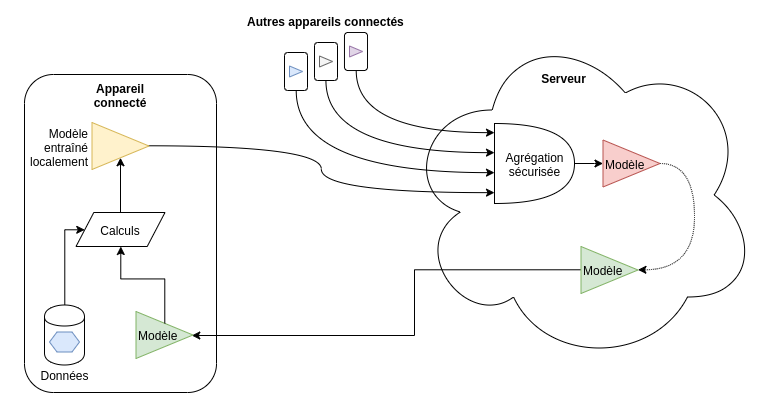
\includegraphics[width=14cm]{decentralize.png}}

Il existe plusieurs manières d'agréger les modèles de client. La première approche est triviale. Considérons que la représentation structurelle du réseau de neurones pour un utilisateur $u$ appartenant à l'ensemble des utilisateurs $U$ soit un vecteur $x_{u}$ de $m$ dimensions. Il suffit que le serveur calcule une moyenne des $x_{u}$. La représentation structurelle $x$ du modèle mis à jour sera alors:

\[
   x = \frac{{}\sum_{u\in U}x_{u}}{|U|}
\]

Malheureusement, dans certaines situations, il est possible de déterminer les activités qu'un utilisateur a exercé en analysant sa contribution dans la mise à jour du modèle. En effet la variation de la structure du modèle est représentative de l'entraînement réalisé sur le téléphone de l'utilisateur. Cependant, dans le contexte de l'apprentissage fédéré, le serveur n'a pas besoin de connaître la contribution individuelle de chacun des utilisateurs mais seulement la moyenne des contributions. Nous sommes donc confrontés à un problème de calcul multipartie sécurisé.

Dans cette étude, nous utiliserons le protocole décrit dans le document \textit{Practical Secure Aggregation
for Privacy-Preserving Machine Learning}\cite{BonawitzPracticalSecureAggregation2017}. Ce protocole se base sur l'algorithme de Shamir\cite{ShamirHowShareSecret1979} qui permet de partager un secret en $n$ secrets indépendants où certaines des parties (ou l'ensemble d'entre elles) sont nécessaires afin de reconstruire le secret initial. L'idée générale de ce protocole est que les clients modifient le vecteur $x_{u}$ en un vecteur $y_{u}$ en ajoutant ou soustrayant des constantes. Ces constantes sont définies entre un utilisateur $u_{1}$ et un utilisateur $u_{2}$ tel que $y_{u_{1}} + y_{u_{2}} = x_{u_{1}} + x_{u_{2}}$. Un chiffrement asymétrique est utilisé pour que les utilisateurs se mettent d'accord sur ces constantes sans que le serveur puisse les déterminer. Nous vous recommandons de lire en détail l'explication du protocole décrit dans la référence citée ci-dessus.

\subsection{La reconnaissance d'activité}

Durant ces dernières années, de nombreuses études ont été menées dans le but de reconnaître des activités physiques. Cependant, la majorité d'entre elles se basait sur l'utilisation de différents capteurs placés à des endroits stratégiques du corps du sujet, comme la cheville, la cuisse ou le mollet par exemple.  \cite{BaoActivityRecognitionUserAnnotated2004}
Cependant, dans un cadre plus concret, couvrir un patient de capteurs dans sa vie quotidienne est peu envisageable. De là vient notre intérêt pour une reconnaissance d'activité non envahissante pour le sujet, grâce à son téléphone mobile. L'analyse sera moins précise qu'une batterie de capteurs mais elle rend l'étude réalisable pour un suivi quotidien non intrusif. Le GPS étant trop peu précis, nous allons nous baser pour cet état de l'art sur l'utilisation de l'accéléromètre du téléphone. \cite{SunActivityRecognitionAccelerometer2010a} De même, les montres et bracelets connectés ne peuvent pas être utilisés pour le moment car leurs mouvements par rapport à l'activité sont trop aléatoires et dépendent trop du sujet étudié.

\subsubsection{Contraintes de l'utilisation d'un accéléromètre}

Pour une analyse non contraignante, le patient ne doit pas s'occuper de positionner son téléphone dans un certain sens dans une poche bien précise, l'analyse se veut naturelle. \newline
Deux problèmes majeurs se posent donc lors de l'utilisation d'un accéléromètre dans la reconnaissance d'activité : 
\begin{itemize}
    \item La position du téléphone : il peut être dans n'importe quelle poche d'un pantalon.
    \item L'orientation du téléphone dans la poche : il peut être dans n'importe quel sens.
\end{itemize}
Ces deux facteurs ont une influence sur les données recueillies par les capteurs et donc sur les résultats obtenus.

Pour résoudre le problème de la position du téléphone, il convient de définir des positions basiques. En effet, un utilisateur lambda va généralement mettre son téléphone dans la poche avant de son pantalon, verticalement. Ce qui permet de définir différentes positions comme : téléphone vers le bas direction intérieur, téléphone vers le bas direction extérieur, téléphone vers le haut direction intérieur et téléphone vers le haut direction extérieur. 
Puis on traite les données en connaissance de la position actuelle. Il est possible aussi de traiter les données de manière générale sans en tenir compte mais l'analyse perd en qualité.

Pour résoudre le problème de l'orientation du téléphone, le principe est d'utiliser l'accélération du mouvement et notamment sa norme, qui elle n'a pas de direction est n'est donc pas sensible à l'orientation du téléphone. 

\subsubsection{Traitement de l'information}

L'accéléromètre d'un téléphone Android renvoie par défaut pour chaque lecture le vecteur d'accélération selon les trois axes orthogonaux A = ($a_{x}$,$a_{y}$,$a_{z}$). \cite{Motionsensors} 
On ajoute à ce vecteur la norme de l'accélération pour obtenir un vecteur 4-dimensions de la forme A = ($a_{x}$,$a_{y}$,$a_{z}$,$\| $$a_{x}$$,$$a_{y}$$,$$a_{z}$$\|$ ).

Les données sont stockées sous la forme de fenêtres pour pouvoir être par la suite traitées. Ces fenêtres sont découpées en plus petites parties, que l'on peut appeler des frames, qui correspondent à au moins un pas. Pour répondre à ce besoin de capturer au moins un pas, les frames sont taillées sur une durée d'une seconde. Pour empêcher tout effet de bord et ainsi capter la notion du temps, il y a un chevauchement de moitié sur ces fenêtres. 

\begin{figure}[!ht]
    \centering
    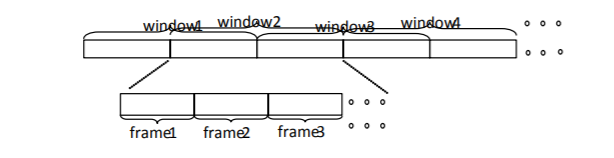
\includegraphics[scale=0.8]{overlapping_explanation.PNG}
    \caption{Fenêtres, frames et chevauchement de moitié            \cite{SunActivityRecognitionAccelerometer2010a}
    }
\end{figure}

\subsubsection{Classification}

Une fois les données d'accélération capturées et stockées, il faut ensuite en extraire certaines fonctionnalités qui seront fournies au classifieur. On peut par exemple isoler des moyennes, des variances, des corrélations ou même l'énergie par transformée de Fourier. Il revient ensuite de décider lesquelles seront choisies en entrée du classifieur sachant que pour chaque composante du vecteur A il est possible d'extraire au moins une fonctionnalité.
Augmenter le nombre de fonctionnalités aura pour effet d'améliorer la précision de l'étude. Cependant, les ressources nécessaires pour obtenir puis utiliser ces données va croître également, ce qui n'est pas conseillé dans le cas où le traitement s'effectue sur mobile et non sur une machine puissante.

A propos des classifieurs, il est possible de mettre en place un apprentissage supervisé comme notamment une machine à vecteur de support (SVM, support vector machine). Le choix dépend pour nous de ce qui est disponible sur mobile actuellement.

\subsection{Les moyens techniques}

Pour prédire l'activité exercée par un patient, nous utilisons un réseau de neurones. Nous avons donc comparé les différentes solutions techniques existantes afin d'en choisir une cohérente avec notre problème. Nous nous sommes confrontés à des problèmes de compatibilité entre les différentes frameworks durant l'implémentation de notre preuve de concept. En effet le modèle a été entraîné avec le framework Tensorflow puis converti en un modèle TensorFlowLite, qui ne permet pas l'entraînement sur téléphone. Comme décrit dans la partie précédente, le federated learning est un domaine de recherche actif. C'est pourquoi les implémentations de ce principe dans les frameworks de machine learning les plus connus n'en est qu'à ses débuts.

\subsubsection{Deeplearning4j}

Deeplearning4j (DL4J) est une librairie Java d'apprentissage profond développé par la fondation Eclipse. Le Java étant le langage de base d'Android, cette librairie est donc compatible avec les téléphones Android et permet donc l'entraînement sur téléphone.\cite{AndroidDeepLearning}

DL4J contient différents modules utiles à la création et l'exploitation de réseaux de neurones. Cette librairie permet notamment l'entraînement d'un modèle directement sur téléphone Android, ce que nous recherchons dans notre cas d'étude. Comme la majorité des frameworks de deep learning, l'entraînement d'un modèle sur DL4J demande de grandes ressources de calculs.

Cette librairie permet l'importation de modèles TensorFlow (basé sur l'API Keras) mais ne permet pas l'exportation vers ce format. Puisque notre modèle est au format TensorFlow / TensorFlow Lite, nous n'avons pas retenu cette solution technique.\cite{EclipsefoundationKerasImportOverview} 

\subsubsection{CoreML}

Core ML est un framework développé par Apple afin d'appliquer certains traitements de machine learning aux données utilisateurs d'iPhones, directement sur leur appareil.

Comme pour DL4J, Core ML repose sur un modèle déjà entraîné qui est perfectionné sur l'appareil. Ce framework s'oriente principalement sur la personnalisation d'un modèle pour correspondre aux données de l'utilisateur. Cette particularité rend Core ML plus efficace dans le traitement de données cohérentes pour un utilisateur. Par exemple, la reconnaissance faciale Face ID (reconnaissance d'un visage unique mais faiblement variable dans le temps) tire parti de Core ML pour affiner le modèle en fonction de ce visage.\cite{MatthijsHollemansTrainingIOSdevice}

L'envoi du modèle Core ML depuis un serveur vers une application installée sur l'appareil représente la norme, mais l'échange inverse, de l'appareil vers le serveur, n'est pas disponible. L'application elle-même utilise le modèle et peut le modifier, mais la nouvelle version du modèle n'est pas conçue pour être partagée ensuite.

Core ML est donc un framework centré sur l'affinage d'un modèle au sein d'une application iOS (et uniquement iOS), sans réunification des différents modèles des utilisateurs. Nous n'avons pas retenu cette solution technique.

\subsubsection{Tensorflow}

Tensorflow est une solution de machine learning développée par Alphabet. La solution est très complète et son API est disponible dans plusieurs langages de programmation. La déclinaison Android de ce framework est TensorFlow Lite. L'entraînement coté serveur de notre cas d'étude utilise Tensorflow puis convertit le modèle en un format TensorFlowLite ce qui permet de faire des prédictions directement sur téléphone.

Cependant Tensorflow Lite ne permet pas le ré-entraînement de ces réseaux directement sur mobile.

C'est pourquoi nous avons choisi d'utiliser l'API Java Tensorflow directement sur Android. Cela nous permet de ré-entraîner nos modèles directement sur l'appareil mobile, puis de renvoyer les mises à jour coté serveur. Nous nous appuyons sur l'application VisionAir qui implémente ce type de solution\cite{DivyanshuSharmaImplementingFederatedLearning}. Les données privées utilisées pour affiner notre modèle restent donc uniquement sur l'appareil de l'utilisateur, seule la structure du modèle est transmise au serveur.

\subsubsection{RSTensorFlow}

RSTensorFlow se positionne comme une version étendue de TensorFlow qui permet d'utiliser toutes les ressources disponibles d'un téléphone android (CPU et GPU). En effet, la version basique de TensorFlow n'utilise que le CPU pour entraîner ses modèles et effectuer des prédictions. \cite{AlzantotRSTensorFlowGPUEnabled2017} \newline
De plus, les noyaux de cette librairie ont été modifiés pour fonctionner avec le framework RenderScript qui permet de paralléliser des calculs à haute performance sous Android. RSTensorFlow rend donc possible l'apprentissage supervisé sur téléphone avec un rendement élevé. 

\subsubsection{Structure de la suite de la publication en prévision}
    Intro : 
        - Rappel au Federated Learning, et donc aux problématiques existantes avec, cf 1.2.2
        - Focus sur la brique de l'aggrégation sécurisée
        - Rappel succinct de Shamir et du protocole dérivé qu'on utilise
    Première partie : 
        - Explications techniques plus détaillées sur le protocole et pourquoi il fonctionne bien 
            - Rapide explication sur le partage de secrets entre plusieurs personnes
            - Insistance sur le double masque
            - Importance du treshold et des locks à chaque étape pour s'assurer que ça continue de fonctionner même quand on drop des clients (assez fréquent avec des mobiles) 
            - Précision sur la possibilité de protéger encore plus (active attack vs honest but curious)
    Deuxième partie : 
        - Zoom in sur notre (celle de La Konch lol) implémentation de l'algo et de comment ça fonctionne
        - Topo sur les mesures de perf en fonction du nombre de clients qui tentent de se connecter (des pertes de gens qui se barrent ?) 
        - Point sur tensorflow 
    Conclusion : 
        - À quel point on est proches d'avoir une chaine de federated learning opérationnelle
        - Problématiques générées par le fait qu'on ait pas réussi à se greffer à l'existant
        - Travail de vraie recherche sur ce qu'on a produit
        - Pistes d'améliorations 

\printbibliography

\end{document}
